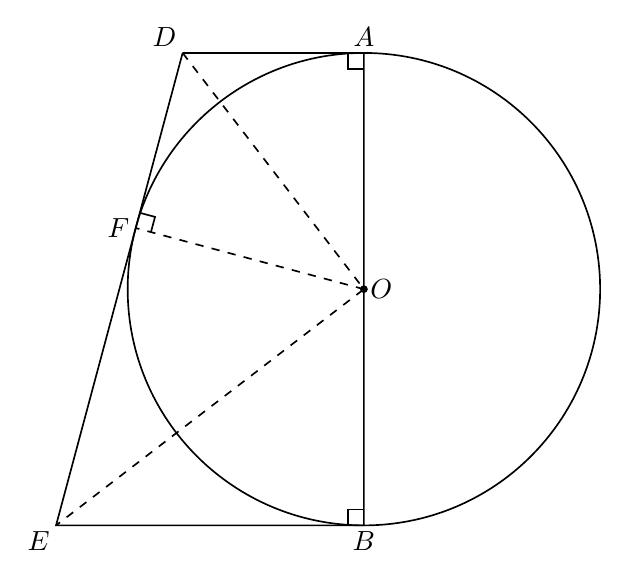
\begin{tikzpicture}[x=1cm,y=1cm,line width=.6pt,font=\normalsize]
\coordinate (O) at (0.0000000000,0.0000000000);
\coordinate (A) at (0.0000000000,3.0000000000);
\coordinate (B) at (0.0000000000,-3.0000000000);
\coordinate (F) at (-2.8977774789,0.7764571353);
\coordinate (D) at (-2.3019809639,3.0000000000);
\coordinate (E) at (-3.9096761185,-3.0000000000);
\draw (O) circle[radius=3cm];
\draw (D)--(A)--(B)--(E)--(D);
\draw[dashed] (D)--(O)--(E) (O)--(F);
\draw (-.2,3)--(-.2,2.8)--(0,2.8);
\draw (-.2,-3)--(-.2,-2.8)--(0,-2.8);
\draw (-2.7045923136,0.7246933263)--(-2.6528285046,0.9178784915)--(-2.8460136698,0.9696423006);
\node[above=2pt,inner sep=0pt] at (A) {$A$};
\node[below=2pt,inner sep=0pt] at (B) {$B$};
\node[above left=2pt,inner sep=0pt] at (D) {$D$};
\node[below left=2pt,inner sep=0pt] at (E) {$E$};
\node[left=2pt,inner sep=0pt] at (F) {$F$};
\node[right=2pt,inner sep=0pt] at (O) {$O$};

% Explicit named circle-center points, painted after all region fills.
\fill (O) circle[radius=1.4pt];
\end{tikzpicture}
